
In this section, we evaluate the efficacy of next-token prediction and chain-of-thought reasoning for verification compared to standard verification approaches. To this end, we compare \genV\ and standard verifiers on a number of reasoning tasks to answer the following questions: (1) How does $\genV$ compare to discriminative verifiers and other approaches? (2) Does unified training of \genV\ improve generation and verification performance? (3) Can {\genV} effectively utilize CoT reasoning to improve its performance? (4)
How does {\genV} scale with model size and inference-time compute?



% \begin{figure}[t]
% \centering
% \footnotesize
%     \begin{tabular}{ |p{16.4cm}| }
%     \toprule

% \multicolumn{1}{|p{16.2cm}|}{
% {\textbf{Problem}: Digimon had its 20th anniversary.  When it came out John was twice as old as Jim.  If John is 28 how old is Jim?}
% } \\
% \midrule
% {\textbf{Solution}: {{Let Jim's age be x when Digimon came out.}} That means John's age is 2x when Digimon came out.\newline
% {20 years ago, \color{red}John's age was 2x - 20 (current age - 20 years) and Jim's age was x - 20 (current age - 20 years).}\newline
% We know that 2x - 20 = 28 (since John's current age is 28)\newline
% 2x = 48\newline
% x = 24\newline
% So, when Digimon came out, Jim was 24. Since it's been 20 years, Jim is now 24 + 20 = 44 years old. {\color{red}The answer is 44.}}\\
% \midrule
% {\textbf{Discriminative RM} score: {\color{red}0.9778}}\\
% \midrule
% {\textbf{\genV-CoT}: Let's verify step by step.\newline
% $\cdots$\newline
% Step 2: {\color{red}20 years ago, John's age was 2x - 20 (current age - 20 years) and Jim's age was x - 20 (current age - 20 years). (Correct)}\newline
% $\cdots$\newline
% Step 6: So, when Digimon came out, Jim was 24. Since it's been 20 years, Jim is now 24 + 20 = 44 years old. \underline{\textbf{\color{blue}(Incorrect)}}\newline
% **Expected Answer:**\newline
% Since John was twice as old as Jim when Digimon came out 20 years ago, and John is 28 now, we can calculate Jim's age. {{Let Jim's age 20 years ago be x.}} {\color{blue}Then we know that 2x = 28 - 20 = 8, so x = 4.} Therefore, Jim's age now is 4 + 20 = 24. {\color{blue}The answer is 24.}\newline
% $\cdots$\newline
% Verification: {\color{blue}Is the solution correct (Yes/No)? No}} \\
% \midrule
% {\textbf{\genV-CoT} (Majority Voting) score: {\color{blue}0.0000}}\\
% \bottomrule
% \end{tabular}
% \caption{
% \textbf{What happens when {\genV} does not catch the mistake in its first pass?} At the end of the step-by-step verification, {\genV}-CoT tends to output a \textbf{\underline{correct}}/\textbf{\underline{incorrect}} token summarizing if the final answer seems wrong, similar to a direct {\genV} that only predicts Yes/No. If {\genV} deems the final answer incorrect, it will attempt to solve the problem again using a reasoning path different from the solution.
% In the example above, even though the step-by-step verification fails to find any mistake, {\genV} gives the problem another try and correctly verifies the solution. Full verification output in \autoref{cot-verifier-example-12-full-text}. This behavior emerges from training on synthetic rationales generated using the prompting format shown in \autoref{prompt-cot-rationale-generation}.}
% \label{cot-verifier-example-main-2}
% \end{figure}





\textbf{Tasks.} We focus on the following tasks and put details about data generation in \autoref{sec:data_details}:
\begin{itemize}[leftmargin=15pt,topsep=1pt,partopsep=1ex,parsep=1ex,itemsep=0pt]
    \item \textbf{Algorithmic reasoning}. We use two difficult string manipulation tasks, namely Last Letter Concatenation~\citep{wei2022chain}
    and Word Sorting from Big-Bench~\citep{suzgun2022challenging}. We train verifiers on  word lists of length \{2,3,4\}, and evaluate their generalization on length \{5,6\}. Note that this is a case of \textit{length generalization} for the verification task.
    % \item \textbf{Last Letter Concatenation}~\citep{wei2022chain}: Given a list of words, the task is to concatenate the last letters of each word (for instance, \textit{``Noah Paul Elisha Rebecca''} $\rightarrow$ \textit{``hlaa''}). We train verifiers on lists of lengths $2-4$, and evaluate them on word lists of length 6. 
    % \item \textbf{Word Sorting}~\citep{suzgun2022challenging} Given a list of words, sort them in alphabetical order. We train verifiers on up to 4-words, and evaluate generalization on 5 word examples.
    \item \textbf{Math reasoning}. We train grade-school math verifiers on the GSM8K dataset from \citet{cobbe2021training} that popularized test-time verification. We evaluate these verifiers on the GSM8K test set as well as their \emph{easy-to-hard generalization} on much harder MATH dataset~\citep{hendrycks2021measuring}, using the same held-out set of 500 MATH problems as \citet{lightman2023let}. We also evaluated model performance on the mathematical tasks in MMLU \citep{mmlu} dataset.
\end{itemize} 

\begin{figure}[h]
    \centering
    \vspace{-0.4cm}
    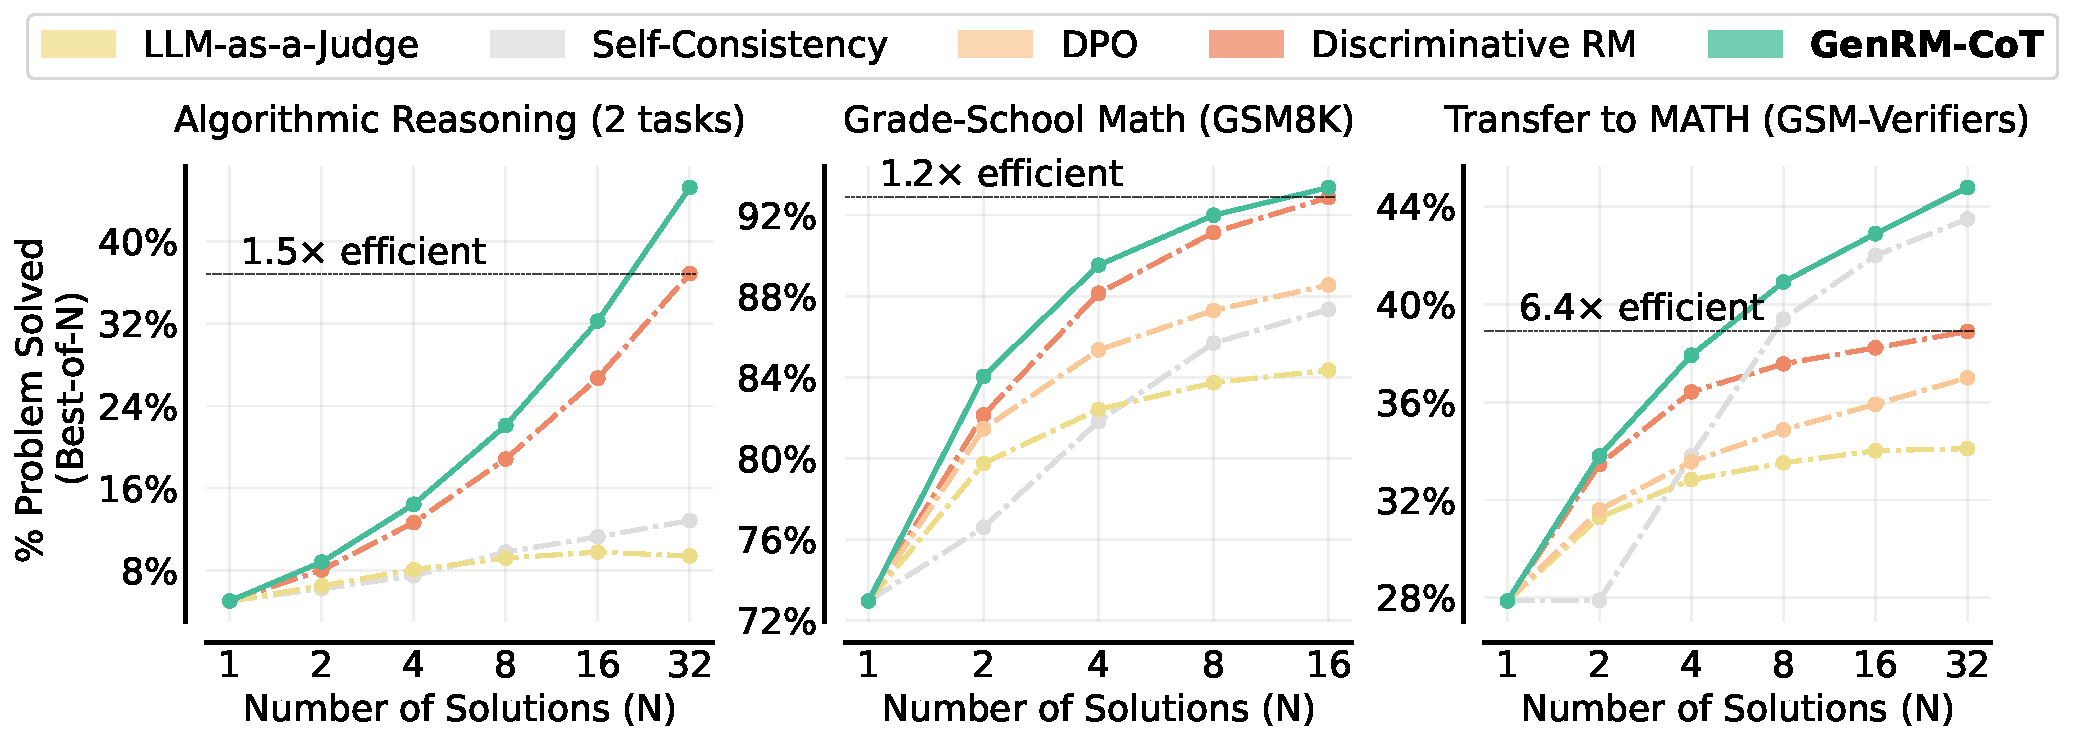
\includegraphics[width=0.92\linewidth]{figures/all_3_final.pdf}
    \vspace{-0.2cm}
    \caption{\footnotesize\textbf{Sample-Efficient Scaling with Generative Verifiers}. \genV-CoT  outperforms other methods, especially for length generalization on algorithmic tasks (Gemma-2B verifiers) and easy-to-hard generalization on MATH (Gemma2-9B verifiers). 
    Specifically, \genV-CoT nearly matches the oracle verifier's Best-of-N performance on algorithmic tasks. On MATH, it matches discriminative verifier's Best-of-32 performance using \boldsymbol{$6.4\times$} \textbf{fewer solutions}.
    }
    \vspace{0.2cm}
    \label{fig:baselines}
% \end{figure}
% \begin{figure}[h]
% \centering
% \vspace{-0.5cm}
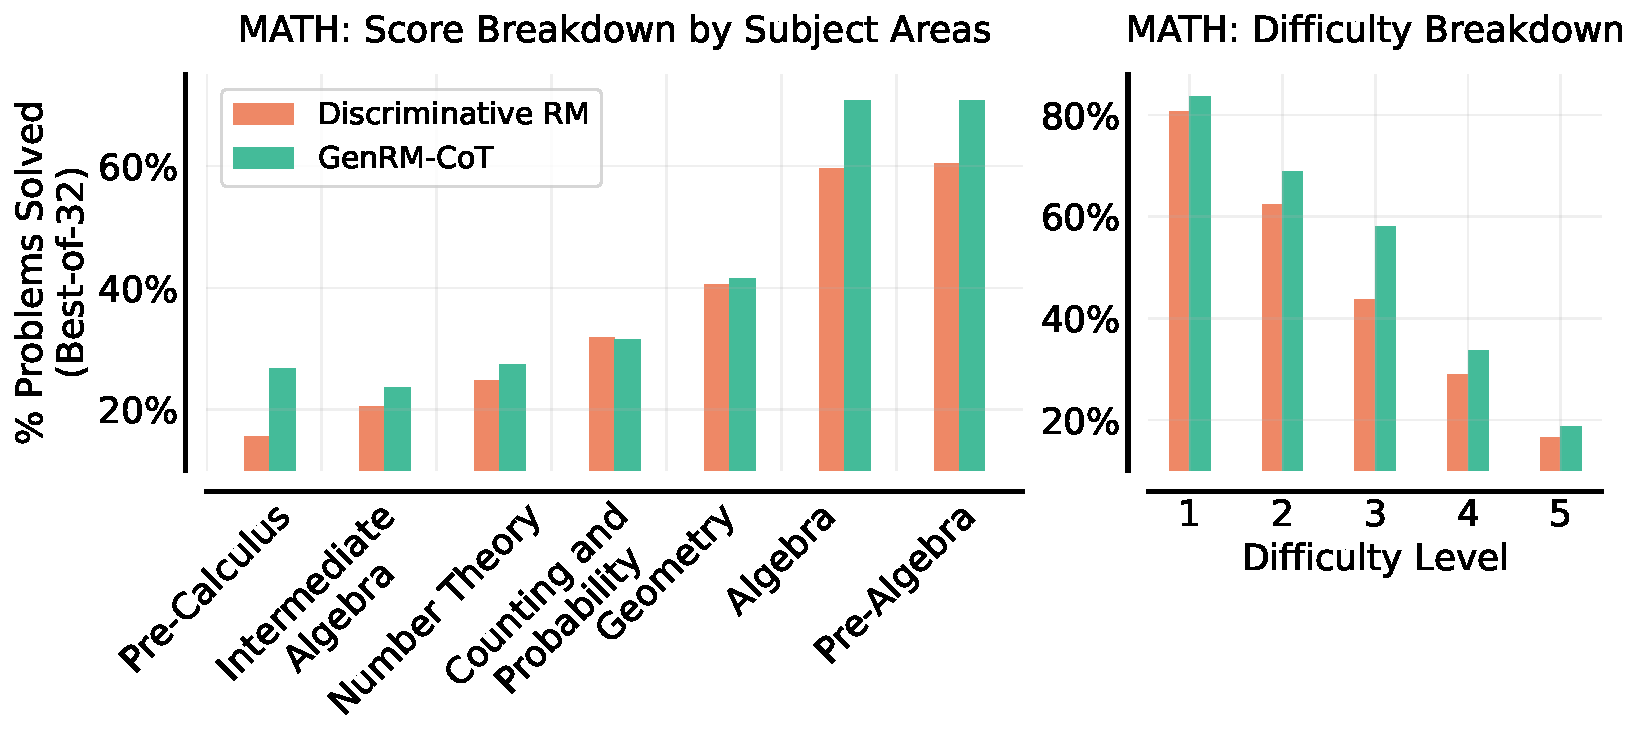
\includegraphics[width=0.85\linewidth]{figures/math_score_breakdown_plot.pdf}
\vspace{-0.3cm}
\caption{\footnotesize\textbf{Easy-to-Hard Generalization on MATH}, with Gemma2-9B verifiers trained only on significantly easier grade-school math problems. Compared to discriminative RMs, \genV-CoT performs especially well on Pre-Algebra, Algebra, and Pre-Calculus, and obtains superior performance across all difficulty levels.
}\label{fig:math_score_breakdown}
\vspace{-0.4cm}
\end{figure}

\textbf{Baselines.} We compare \genV\ to the following verification approaches: 
\begin{itemize}[leftmargin=15pt,topsep=1pt,itemsep=0.2ex,partopsep=1ex,parsep=1ex,itemsep=0pt]
    \item \textbf{Discriminative RM}~\citep{cobbe2021training} or ORM is the prevalent approach for training verifiers for test-time re-ranking on reasoning tasks~(\secref{sec:back}), and serves as our main baseline.
    \item \textbf{LLM-as-a-Judge}~\citep{zheng2024judging} uses an off-the-shelf pretrained LLM for verification. To do so, we use a CoT prompt to produce 32 verification rationales that is used for correctness prediction and pick the majority-vote correctness answer.
    \item \textbf{DPO}~\citep{rafailov2024direct}: Following \citet{hosseini2024v}, we use this preference optimization approach for training verifiers on preference pairs with incorrect and correct solutions. 
    \item \textbf{Self-consistency}~\citep{wang2022self}: A simple approach to use test-time compute \emph{without} verifiers: sample multiple solutions from the LLM generator and pick the most common answer.
\end{itemize}
Note that self-consistency and test-time verification are complementary approaches, and can be often combined via weighted self-consistency to further boost performance, as shown in \autoref{fig:weighted_sc_on_math}.

\textbf{Evaluation protocol.} Following \citet{cobbe2021training, lightman2023let}, we primarily use \textbf{Best-of-N} performance in terms of the percentage of problems solved using a fixed generator~(\secref{sec:back}) with learned verifiers, and report average accuracy on the test set. %Best-of-N evaluates what fraction of solutions chosen by the verifier are correct. 
We also report test \textbf{RM accuracy}, which measures whether the verifier accurately classifies incorrect and correct solutions. While these two metrics are correlated, RM accuracy only evaluates the verifier's point-wise accuracy, while Best-of-N evaluates the verifier's ability to rank solutions for choosing the correct one. %fraction of solutions chosen by the verifier that are correct.
% its group-wise ranking performance.

\textbf{Models \& Training.} For training verifiers, we use open-weights Gemma models~\citep{gemma, team2024gemma}, specifically Gemma-2B for algorithmic tasks, and Gemma 2B, 7B, and Gemma-2 9B for GSM8K. For solution generation as well as LLM-as-a-Judge, we use Gemma 2B for algorithmic tasks and Gemini 1.0 Pro~\citep{team2023gemini} for GSM8K. For verification CoT rationales, we generate oracle rationales for algorithmic tasks programmatically~(\autoref{tab:synthetic}); for GSM8K, we generate synthetic rationales using Gemini 1.0 Pro with reference-guided grading~(\autoref{prompt-cot-rationale-generation}).  %We use the label `Verification Only' to indicate generative verifiers trained using only verification data ($\lambda=0$). 
See \autoref{sec:hyper-parameter-gen-rm} for hyperparameter details.

\subsection{Generative Verifiers Outperform Standard Verification Approaches}
% This shows that the next-token-prediction loss allows \genV\ to tap into the capabilities of pretrained Gemma models more effectively.

\genV\ outperforms LLM-as-a-Judge and DPO verifiers~(\autoref{fig:overall-result}), while performing comparably or slightly better than discriminative verifiers~(\autoref{fig:gen_rm}). \genV-CoT substantially improves the Best-of-N performance over \genV. In particular, on the algorithmic tasks with oracle verification CoTs, \genV-CoT nearly \emph{matches} the oracle verifier performance. 

On GSM8K, \genV-CoT consistently outperforms other methods~(\autoref{fig:baselines}, middle), even though the synthetic CoT rationales for training may contain errors. Qualitatively, {\genV-CoT} is able to detect subtle reasoning errors that are missed by discriminative or direct \genV\ verifiers~(see \autoref{cot-verifier-example-main-1},  \ref{math-transfer-cot-verifier-example-main-figure}, and \ref{cot-verifier-example-main-3}). 
% \ref{cot-verifier-example-main-2},

\begin{table}[h]
\vspace{-0.2cm}
    \centering
    \begin{tabular}{lcccc}
        \toprule
        \textbf{MMLU Dataset} & \textbf{Base Model (Pass@1)} & \textbf{Disc-RM} & \textbf{GenRM-CoT} & \textbf{Improvement} \\
        \midrule
        elementary\_mathematics & 80.1\% & 90.6\% & \textbf{91.1\%} & \textcolor{blue}{+0.5\%} \\
        high\_school\_mathematics & 52.2\% & 74.8\% & \textbf{76.1\%} & \textcolor{blue}{+1.3\%} \\
        college\_mathematics & 47.6\% & 53\% & \textbf{56.1\%} & \textcolor{blue}{+3.1\%} \\
        abstract\_algebra & 37.9\% & 50\% & \textbf{53.50\%} & \textcolor{blue}{+3.5\%} \\
        \bottomrule
    \end{tabular}
    \caption{\textbf{Performance of different methods on math tasks from the MMLU \citep{mmlu} dataset.} The evaluation uses an easy-to-hard generalization setting, where the verifier is trained only on grade school math. We highlight the absolute improvement of GenRM-CoT over the Disc-RM baseline. Notably, Gen-CoT demonstrates stronger performance across all tasks, with the improvements being more significant on harder tasks.}
    \label{tab:mmlu-table}
\end{table}

\begin{figure}[t]
\centering
\vspace{-0.2cm}
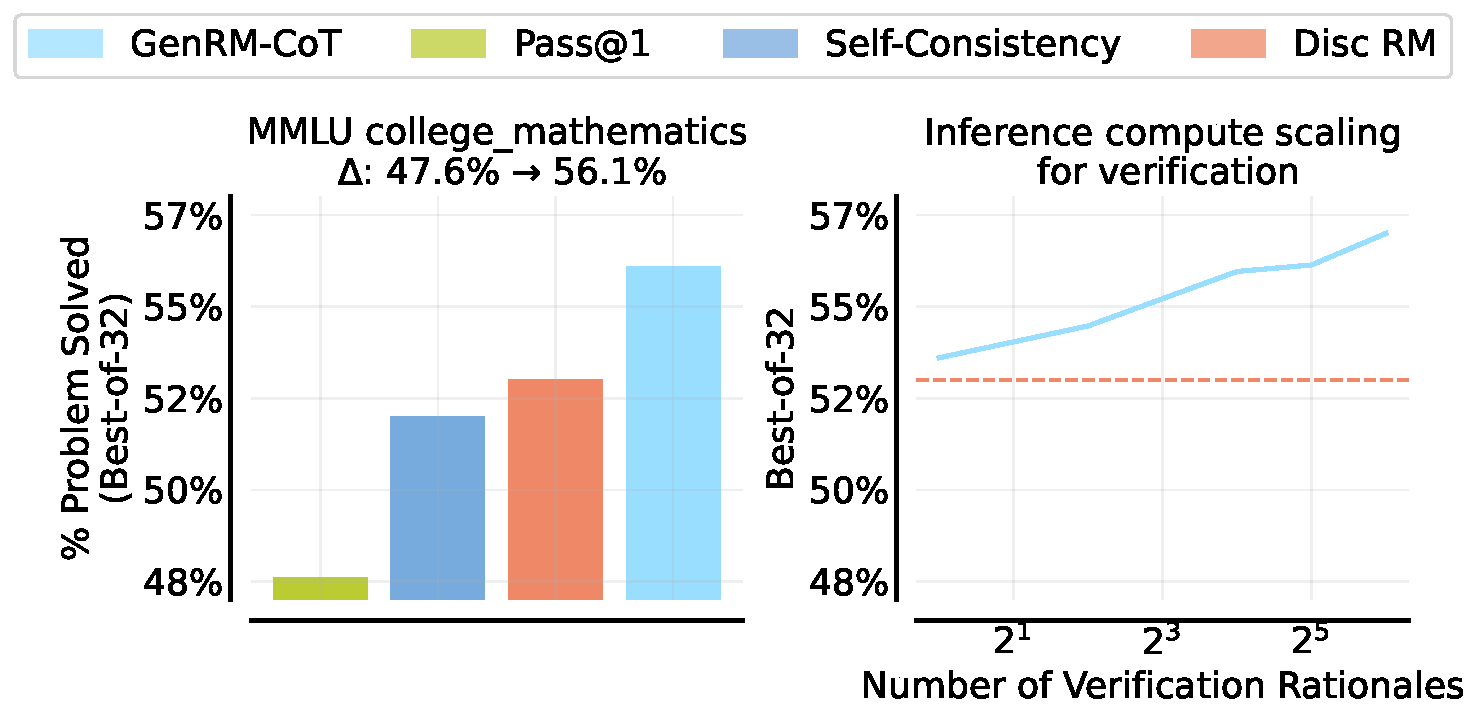
\includegraphics[width=0.7\linewidth]{figures/mmlu_figure.pdf}
\centering
\vspace{-0.2cm}
\caption{\textbf{Transfer to MMLU College Mathematics} (GSM Verifiers), using Best-of-32 evaluation, with solutions generated from Gemini 1.0 Pro. On college-level mathematics, even using a single verification rationale with \genV-CoT can outperform Discriminative RM. Best-of-32 based on discriminative RM yields a performance of $53.0\%$; as for \genV-CoT (using 32 majority votes), Best-of-32 gives $56.1\%$.
}
\vspace{-0.4cm}
\label{fig:mmlu-college-math}

\end{figure}

\textbf{Easy-to-Hard Generalization}.  Without any training on MATH, \genV-CoT results in a $6.4\times$ better sample efficiency than discriminative verifiers as we increase the number of solutions to verify, and surpasses the strong self-consistency baseline~(\autoref{fig:baselines}, right). While \citet{sun2024easy} demonstrate that discriminative verifiers trained on easy MATH problems can generalize to harder MATH problems, \genV-CoT exhibits a much stronger generalization from \emph{grade-school} math problems to \emph{high-school competition} problems in MATH~(see \autoref{fig:math_score_breakdown} for a score breakdown by subject areas and difficulty levels) and college-level math in MMLU (see \autoref{tab:mmlu-table}).

\begin{wrapfigure}{r}{0.40\textwidth}
\vspace{-1.0cm}
\centering
\begin{minipage}{0.40\textwidth}
    \centering
    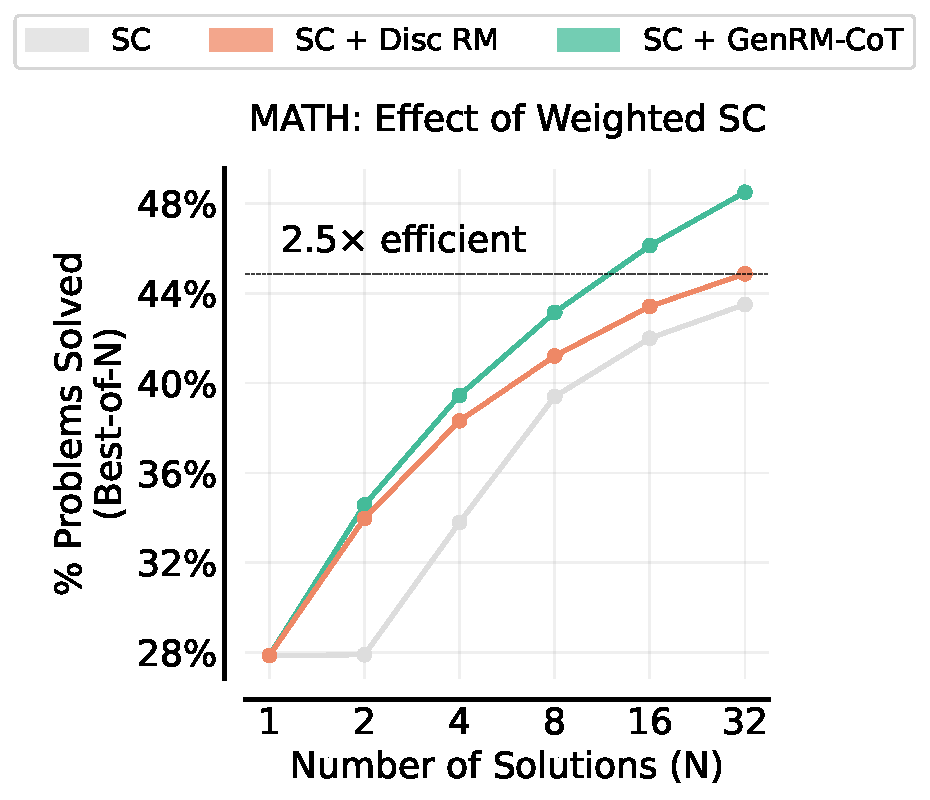
\includegraphics[width=0.95\linewidth]{figures/figure_weighted_sc_math.pdf}
    \vspace{-0.2cm}
    \captionof{figure}{\footnotesize\textbf{Weighted Self-Consistency} on MATH.}
    \label{fig:weighted_sc_on_math}
\end{minipage}
\vspace{-0.8cm}
\end{wrapfigure}

\textbf{Leveraging Self-Consistency with Verifiers}. Self-consistency and test-time verification can be easily combined to boost Best-of-N performance. To do so, we use weighted self-consistency or majority-voting~\citep{uesato2022solving, improving-llm-finetune-for-math, sun2024easy} where we weight each solution according to the verifier's score, and select the final answer with the largest weight (see \autoref{sec:weighted-sc-details} for details).
\autoref{fig:weighted_sc_on_math} shows that weighted SC can indeed improve the vanilla self-consistency (SC); in particular, weighted SC based on \genV-CoT requires \textbf{2.5x fewer solutions} than its counterpart based on Discriminative RM to reach the same performance.
\vspace{-0.4cm}
\subsection{Synergy Between Generation and Verification}
\label{sec:unification}

\begin{figure}[t]
    \centering
    \vspace{-0.3cm}
    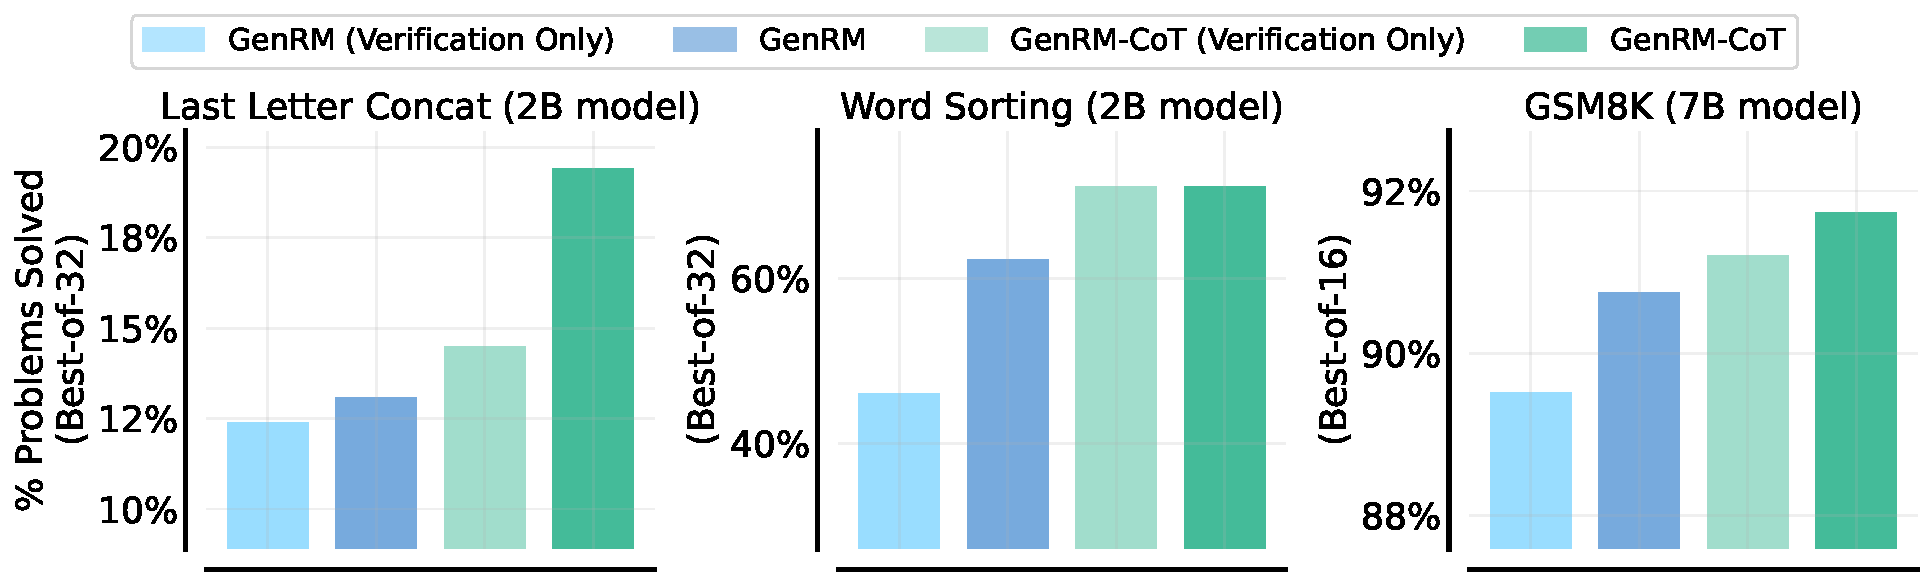
\includegraphics[width=0.9\linewidth]{figures/sft_on_correct_solns_improves_direct_genrm_iclr.pdf}
    \vspace{-0.2cm}
    \caption{\textbf{SFT on correct solutions enhances verification}, both for {\genV} and \genV-CoT, across all tasks. `Verification Only' corresponds to verifiers trained only on verification data, by setting $\lambda=0$ in \eqref{eq:co-train}. The y-axis of each figure starts from the pass@1 performance of the base generator for each task.
    %With or without CoT in verification, generative verifiers treat both generation and verification as next-token prediction, and become better when we simply add the task of generating correct solutions to its training data mixture.
    }
    \label{fig:unification-gen-verify-helps}
    \vspace{0.15cm}
    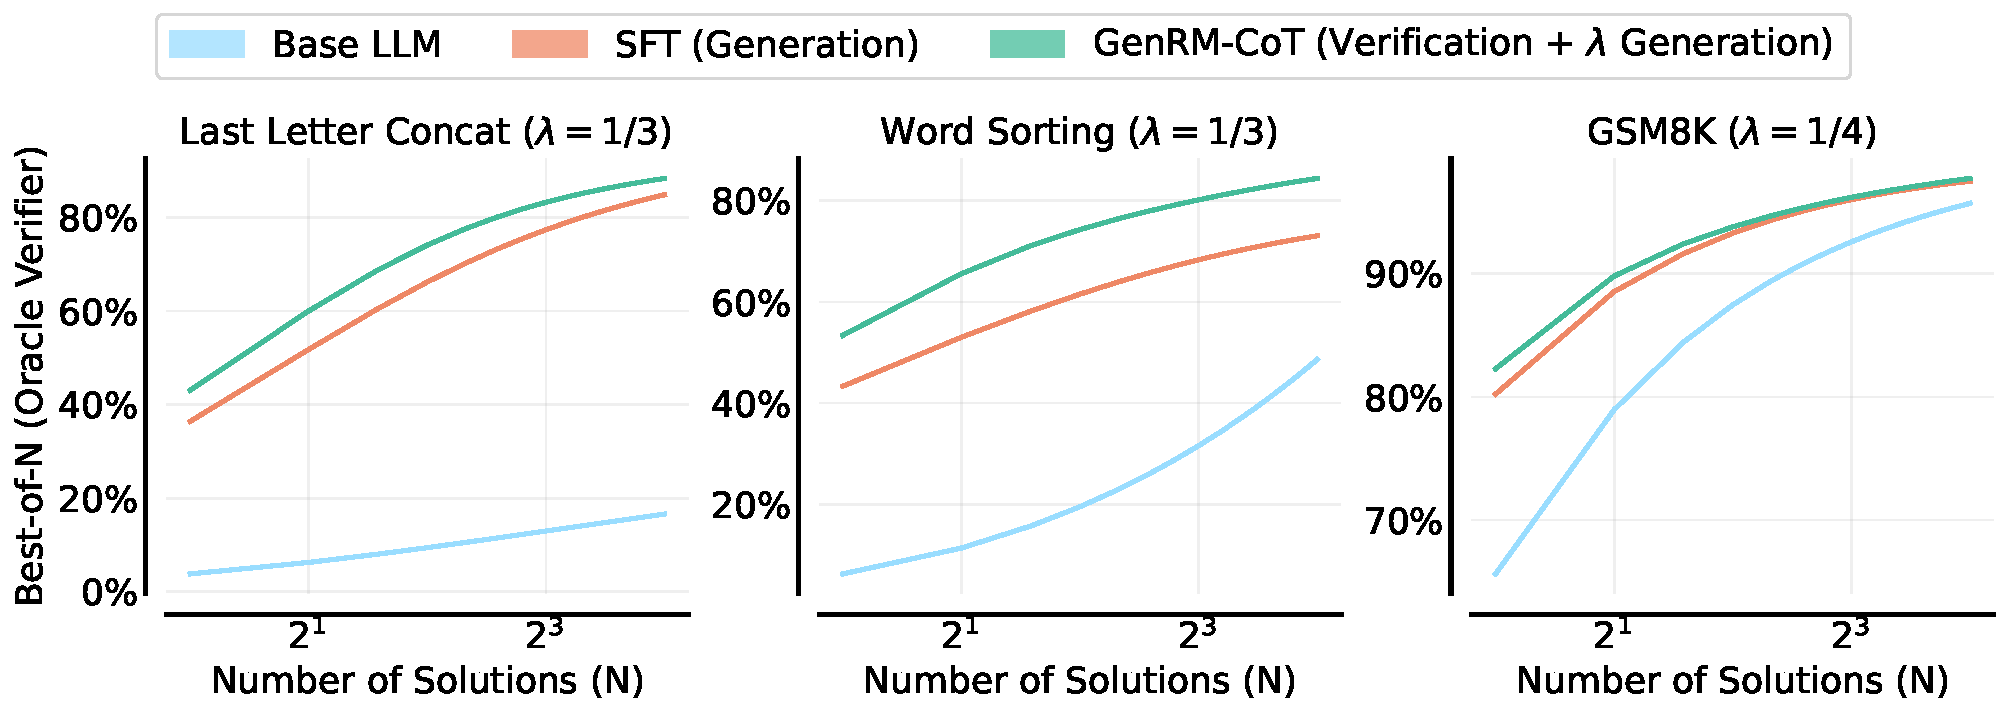
\includegraphics[width=0.9\linewidth]{figures/si_figure.pdf}
    \vspace{-0.15cm}
    \caption{\textbf{Unifying generation and verification boosts generation performance} compared to SFT on correct solutions, in terms of Best-of-N with oracle verifier. The improvement is larger on algorithmic tasks, which use ground-truth verification data, than on GSM8K that relies on synthetic rationales, which may be inaccurate.}
    \vspace{-0.3cm}
    \label{fig:unification-gen-verify-helps-with-generation}
\end{figure}


Unifying solution generation with verification, as done by \genV\ using next-token prediction, consistently improves verification performance across all tasks, as illustrated in \autoref{fig:unification-gen-verify-helps}. This improvement is observed for both direct and CoT-based generative verifiers, suggesting that teaching the verifier to imitate correct solutions generally helps. However, adding too much solution generation data can decrease  verification performance of \genV~(\autoref{fig:impact-of-lambda}). 

Incorporating CoT verification data into the generator's training mix  leads to better solution generation performance for the \genV-CoT verifier itself, as evidenced in \autoref{fig:unification-gen-verify-helps-with-generation} by the improved Best-of-N scores with the oracle verifier (Pass@N). This suggests that teaching a generator to perform CoT verification using next-token prediction can deepen its understanding of the generation process itself. Overall, unifying solution generation and verification is mutually beneficial.
\vspace{-0.4cm}
\subsection{Scaling Model Size and Inference-time Compute}

\begin{figure}[t]
\vspace{-0.4cm}
\centering
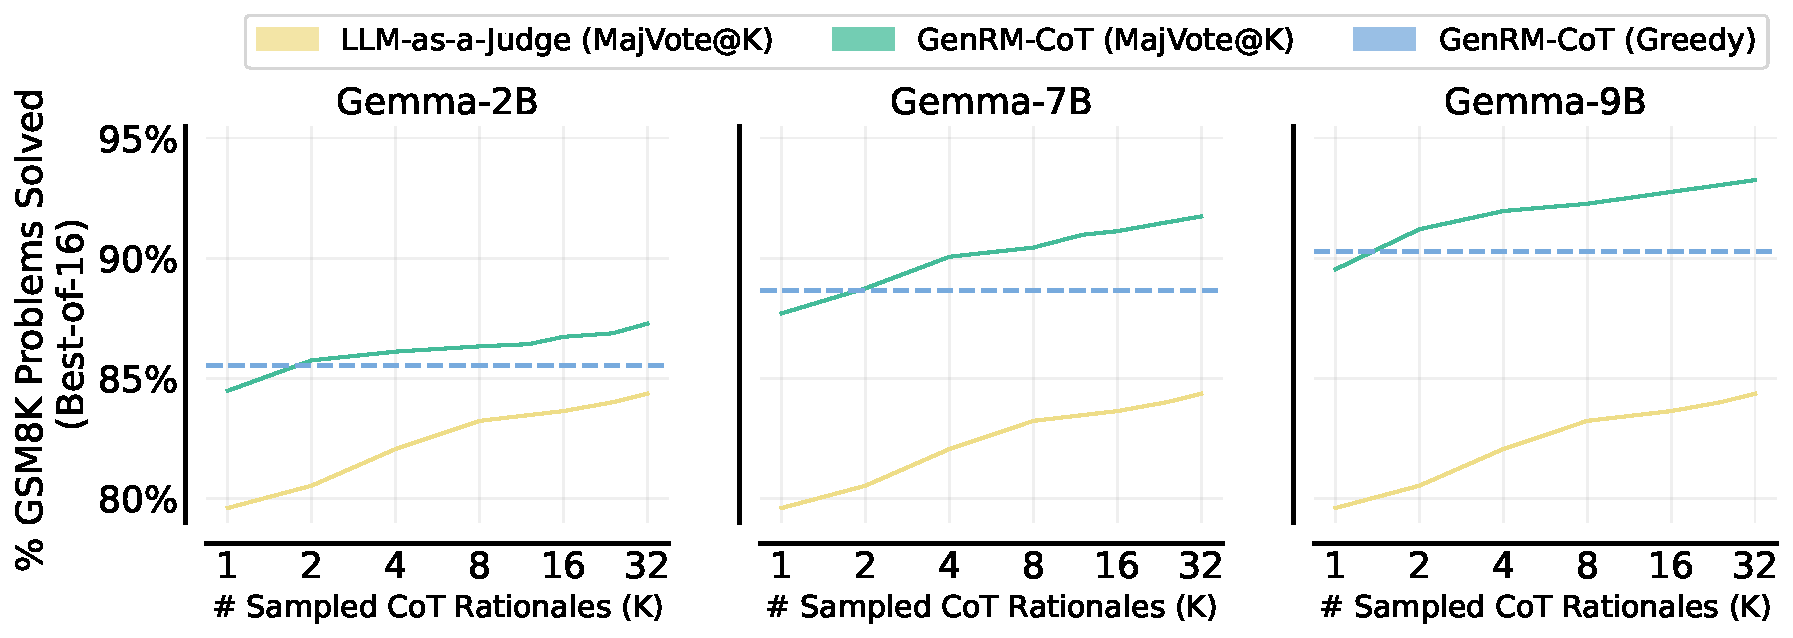
\includegraphics[width=0.9\linewidth]{figures/inference_compute_scaling_gsm_iclr.pdf}
\vspace{-0.2cm}
\caption{\textbf{Scaling Inference-time Compute for Verification} on GSM8K. By posing reward modeling as next-token prediction, \genV-CoT can utilize Chain-of-Thought and Majority Voting, to turn additional test-time compute into higher percentage of problems solved under Best-of-N. 
% The more capable the base model, the more effective inference-time compute scaling seems to become.
Here, the horizontal line corresponds to performance of \genV-CoT verifier with greedy decoding in Eq~\eqref{eq:cot-reward}. 
%\todo{Update this plot with 32 votes to put GSM and MATH results (either transfer or training) side by side.}
}\label{fig:inference_compute_scaling}
% \end{figure}
% \begin{figure}[h]
% \centering
\vspace{0.2cm}
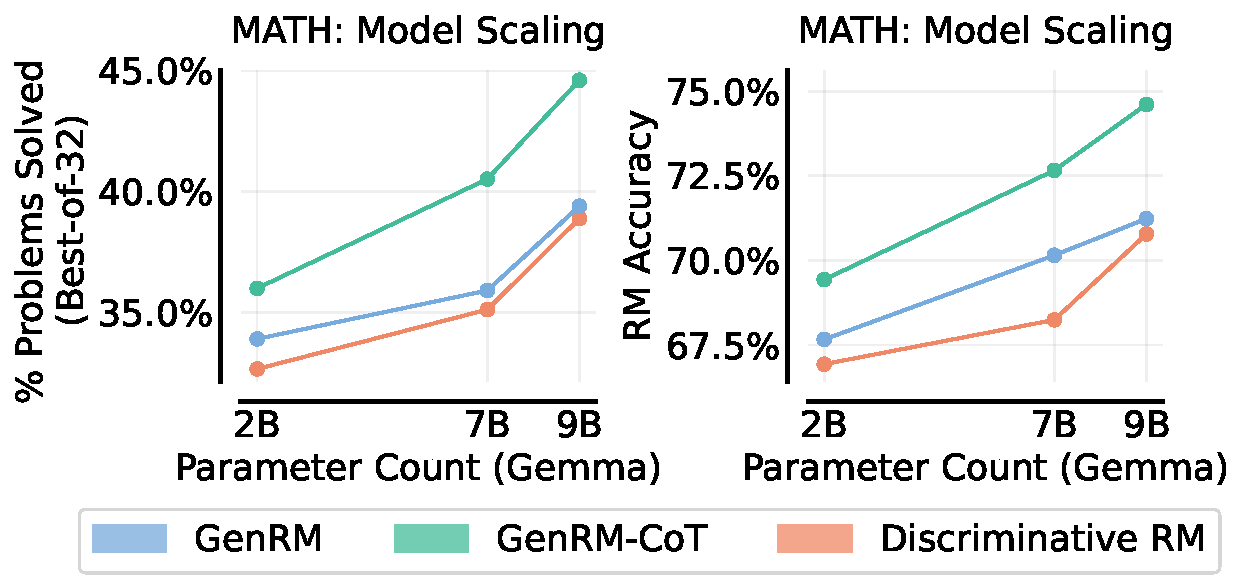
\includegraphics[width=0.7\linewidth]{figures/math_model_scaling_with_test_acc_iclr.pdf}
\vspace{-0.2cm}
\caption{\textbf{Model Scaling for Generative Verifiers.} We evaluate MATH performance of Gemma 2B, 7B, and Gemma2 9B verifiers trained on GSM8K. We observe positive scaling trends for {\genV} (direct) and {\genV}-CoT as well as Discriminative RM, both for (\textbf{Left}) Best-of-N performance, and (\textbf{Right}) RM accuracy on the test set. Generative verifiers outperform discriminative counterparts in all model regimes.
}\label{fig:model_scaling}
\vspace{-0.25cm}
\end{figure}

\textbf{Scaling Test-Time Compute with \genV-CoT} can be done by sampling multiple CoTs and applying majority voting, as described in Eq~\eqref{eq:gen-rm-maj-voting}. As shown in \autoref{fig:inference_compute_scaling},  \genV-CoT verifier's performance scales gracefully with number of votes at test time, under all three Gemma model sizes (2B, 7B, 9B), outperforming greedy decoding performance within 2 votes. Notably, across model scales, the finetuned \genV-CoT verifier outperforms LLM-as-a-Judge , which also utilizes the same CoT approach and number of majority votes, but prompts a more capable Gemini 1.0 Pro model than Gemma models which we finetune as verifiers.



\textbf{Scaling model size.} In \autoref{fig:model_scaling}, we show that generative verifiers, especially \genV-CoT, perform better than discriminative RMs across model sizes, both in terms of reward modeling accuracy and Best-of-N performance.  Intuitively, bigger models are more capable of text generation, allowing {\genV}-CoT finetuning to better tap into its chain-of-thought reasoning ability for verification. Furthermore, these results demonstrate that larger models generalize better using the same data, which matches what we expect from scaling model parameter counts under the next-token prediction loss.

\begin{figure*}[t]
\centering
\begin{minipage}{0.4\textwidth}
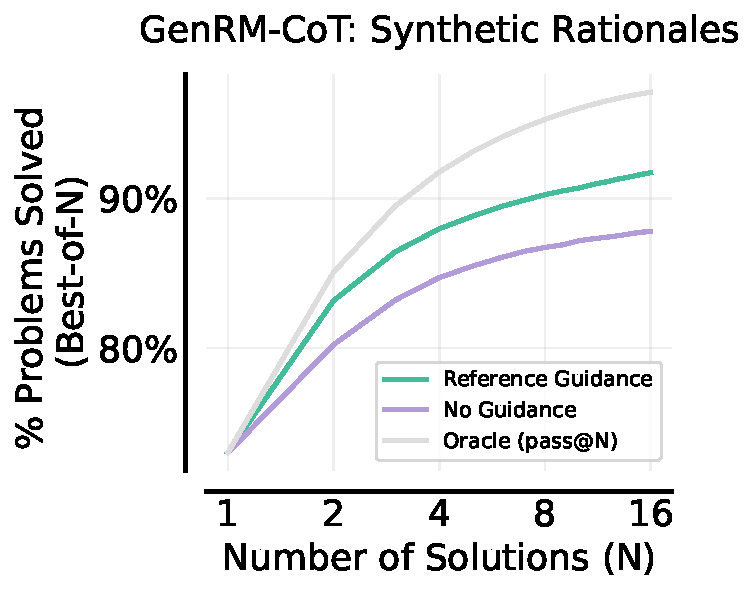
\includegraphics[width=\linewidth]{figures/gsm_ablating_reference_guidance.pdf}
\caption{
\footnotesize\textbf{Quality of synthetic rationales matters}. Using reference guidance for synthetic rationale generation is crucial for {\genV}-CoT to perform well on GSM8K: 91.7\% with guidance vs. 87.8\% without for Gemma-7B verifiers.}
\label{fig:gsm-ablating-reference-guidance}
\end{minipage}
\hfill
\begin{minipage}{0.56\linewidth}
\vspace{-0.6cm}
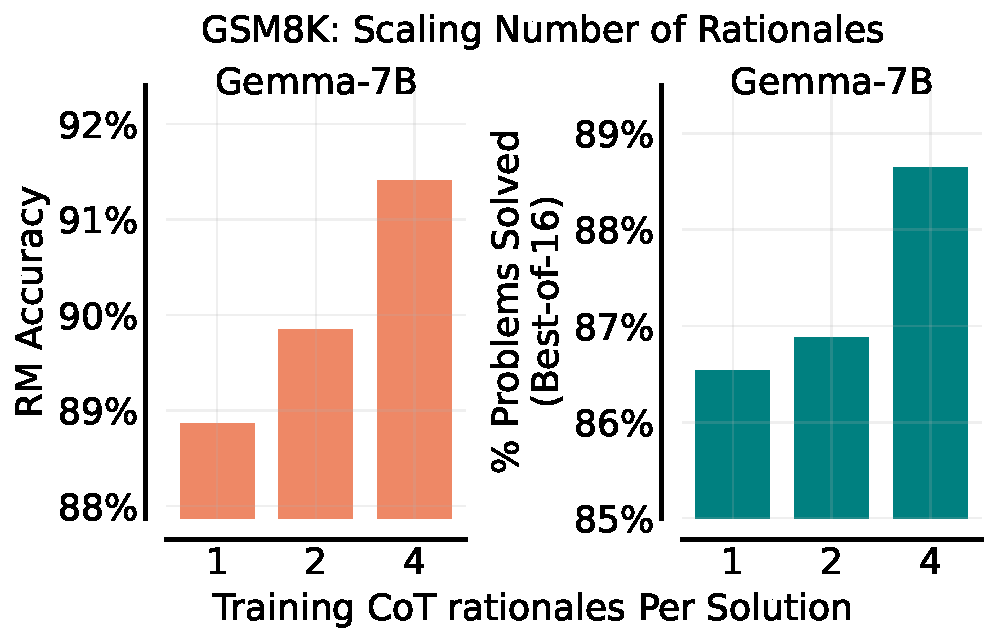
\includegraphics[width=\linewidth]{figures/cot_greedy_critique_scaling.pdf}
\caption{\footnotesize\textbf{Quantity of synthetic rationales matter}. Scaling the number of rationales per solution for \genV-CoT on GSM8K improves both RM accuracy and Best-of-N performance. Here, we use fine-tuned Gemma-7B verifier, with greedy decoding at inference~\eqref{eq:cot-reward}.
}
\label{fig:rationale_scaling}
\end{minipage}
\vspace{-0.3cm}
\end{figure*}


\vspace{-0.1cm}
\subsection{Synthetic Rationales: Quantity and Quality Matter}
\vspace{-0.1cm}



Our results on math reasoning tasks indicate that CoT
verifiers can outperform discriminative and direct verifiers without requiring human-written verification rationales, highlighting the potential of LLM-generated rationales.
We find that both the quality and quantity of these synthetic rationales matter. 
As shown in \autoref{fig:gsm-ablating-reference-guidance},
using reference-guided grading during rationale generation~(\S\ref{sec:cot-verifier}) significantly improves verification performance. Furthermore, using multiple rationales per solution also improves performance, as shown in \autoref{fig:rationale_scaling}. We suspect that this is because model-generated rationales may contain errors, such that training on multiple rationales per solution can result in an ``ensembling'' effect that prevents overfitting to such errors~\citep{zhang2024transcendence}.

Importantly, unlike prior work, our results on math reasoning tasks do not require a more capable model~\citep{ankner2024critique, improve-rm-synthetic-critique} or humans~\citep{critic-gpt, self-critique-models} for generating verification rationales: we use the same model (Gemini 1.0 Pro) to both generate solutions to verify and synthetic verification rationales for training.


\begin{figure}[t]
% \setlength\extrarowheight{3pt}
% \vspace{-0.2cm}
\footnotesize
\centering
\begin{tabular}{ |p{16.4cm}| }
\toprule

\multicolumn{1}{|p{16.2cm}|}{
{\textbf{Problem}: Carol spends 4 hours writing a song, half that much time recording it, and 90 minutes editing it. What percentage of her total work time did she spend editing?}
} \\
\midrule
{\textbf{Solution}: Half of 4 hours is 2 hours. So the time spent recording is 2 hours. Add the editing time of 90 minutes and the total time for the entire project is 4 + 2 + 1.5 = 7.5 hours. {\color{red}That means she spent (90 / 7.5) * 100 = 12\% of the total time editing.} The answer is 12.
} \\
\midrule
{\textbf{Discriminative RM} correctness score: {\color{red}0.8414}}
\\
\midrule
{\textbf{\genV-CoT}: Let's verify step by step. \newline $\cdots$ \newline
Step 3: {\color{red}That means she spent (90 / 7.5) * 100 = 12\% of the total time editing.}\newline
Expected Answer: {\color{blue}Incorrect. The editing time should be in hours, so it should be (1.5 / 7.5) * 100 = 20\%.}\newline

Verification: {\color{blue}Is the answer correct (Yes/No)? No}
} \\
\midrule
{\textbf{\genV-CoT (Majority Voting)} score: {\color{blue}0.2498}}
\\
\bottomrule
\end{tabular}
\caption{
\textbf{An example where \genV-CoT catches a subtle mistake} that the discriminative verifier is unable to catch.
The candidate solution did not convert 90 minutes into 1.5 hours before dividing it by 7.5. However, the discriminative verifier was not able to detect this mistake likely because the solution does still appear to produce a valid-sounding percentage 90/7.5 = 12. Our proposed GenRM-CoT model is able to identify this mistake using step-by-step generative verification.
The full verification output can be found in \autoref{cot-verifier-example-10-full-text}. 
}
% \vspace{-0.3cm}
\label{cot-verifier-example-main-3}
\end{figure}
